% =============================================
% Part 0.0 编辑个人信息
% =============================================

\newcommand{\department}{计算机系}		%在这里修改系别
\newcommand{\major}{大数据}				%在这里修改专业
\newcommand{\class}{大数据1701}					%在这里修改班级
\newcommand{\name}{	张丹颖		}			%在这里修改姓名
\newcommand{\stuid}{ 2017011760			}				%在这里修改学号
\newcommand{\newdate}{2018-12-12			}				%在这里修改日期 yyyy-mm-dd
\newcommand{\loc}{			}					%在这里修改地点

% =============================================
% Part 0.1 编辑课程信息
% =============================================
\newcommand{\newcourse} {数据结构\LARGE{(C)}} %在这里修改成课程名称
\newcommand{\newtitle}{图的生成与操作} %在这里修改实验项目
\newcommand{\exptype}{计算机}

\newcommand{\grades}{}
\newcommand{\group}{无}

\newcommand{\tutor}{丁濛}
\newcommand{\onespace}{\hspace{1em} }
\begin{document}
\begin{titlepage}
	\centering
	\vspace*{1cm}
	{\fontsize{34pt}\baselineskip 实\onespace 验\onespace 报\onespace 告}\\
	\vspace{2cm}
	\fontsize{19pt}\baselineskip
	\makebox[30mm]{课程名称:}
	\underline{\makebox[75mm][c] {\newcourse} }
	\vskip 0.3cm
	\makebox[30mm]{实验项目:}
	\underline{\makebox[75mm][c] {\newtitle }}\\
	\vskip 0.3cm
	\makebox[30mm]{实验仪器:}
	\underline{\makebox[75mm][c]{PC }}\\%在这里修改实验仪器
	\vskip 1cm

    \begin{table}[!htbp]
      \centering
      \sihao
      \begin{tabular}{| c | c | c | c | c | c |}
      	\hline
        项目 & 报告格式 & 写作质量 & 逻辑、注释质量、思想描述 & 复杂度分析 & 合计\\
        \hline
        
        百分比(\%) & 15 & 25 & 40 & 20  & 100 \\
        \hline
        得分	& {\gradeFormat } & {\gradeCode } & {\gradeComment}   & {\gradeComplex} & {\gradeTotal} \\
        \hline
      \end{tabular}
    \end{table}
     \Comments
    	
	\vskip 2cm

        \begin{table}[!tbhp]
            \centering
            \sanhao
            \begin{tabular}{ll}
                系\hspace{2em}别:	&	 \underline {\makebox[60mm][c]	{\department} 	} \\
                专\hspace{2em}业:	&	 \underline {\makebox[60mm][c] {\major}		} \\
                班级姓名:		&	\underline {\makebox[60mm][c] {\class\ \name\ }		} \\
                日\hspace{2em}期:	&	 \underline {\makebox[60mm][c]	{\newdate} 	} \\
                成\hspace{2em}绩:	&	 \underline {\makebox[60mm][c] {\grades}		} \\
                同组成员:		&	\underline {\makebox[60mm][c] {\group}		} \\
                指导教师:		&	\underline {\makebox[60mm][c] {\tutor}		} \\
            \end{tabular}
        \end{table}


%    
%    

\end{titlepage}

\newpage
% =============================================
% Part 2 Main document
% =============================================
\xiaosihao
\section{实验目的}
\begin{enumerate}
\item 掌握图的邻接矩阵和邻接链表两种表达方式;
\item 能够根据输入建立一张图,并可以获取图中的结点以及边的相关信息;(验证)
\item 熟练掌握图的BFS和DFS过程;掌握寻找无向图极大连通分量的过程;(验证)
\item 掌握最小生成树算法(Kruskal); 掌握Dijsktra算法;(验证)
\item 会计算一个无向图的割点;
\item 体会图在实际应用中能够解决的问题(设计、综合)。
\end{enumerate}

\section{实验内容}
\subsection{项目一}
根据输入,建立一张无向图(可以采用任何一种图结构)。根据你建立的图,实现如下功能:
\begin{enumerate}
\item 获得给定顶点所有的邻接边;
\item 计算一个顶点的度。

\end{enumerate}

\subsection{项目二}
根据输入,建立一张有向图(可以采用任何一种图结构)。根据你建立的图,实现如下功能:
\begin{enumerate}
\item 获得给定顶点所有的邻接边;
\item 计算一个顶点的入度和出度。
\end{enumerate}

\subsection{项目三}
对于给定的一张图,分别对其进行BFS和DFS遍历。要求输出每个结点的前驱结点,首次访问时间以及结束时间(被标记为BLACK的时间)。

\subsection{项目四}
完成实验平台上实验四的题目

\section{实验过程}
\subsection{项目1}
大致思想 :采用邻接矩阵的存储方式,Node结构体中,存放度数degree,结点名字data 和存放邻接点的一维数组*AdjList;用一个数组NodeList存储所有节点。输入每条边的信息时,将对应下标结点的信息填入。再依次打印即可
\subsubsection{实验步骤}
\begin{enumerate}
\item createAdjGraph()函数构建无向图,复杂度O(V+E),V是顶点数,E是边数。
\item display()打印所有顶点的所有邻接边和度数。复杂度O($V^2$),V是顶点数。       遍历每个点,对于每个点,根据度数挨个打印邻接数组中的邻接点。
\end{enumerate}

\subsubsection{必要代码}
\lstinputlisting[language=C++]{code/1/main.cpp }
\lstinputlisting[language=C++]{code/1/UnDirectedGraph.h}
\subsubsection{实验结果}如图1
	\begin{figure}[!bthp]
	\centering
        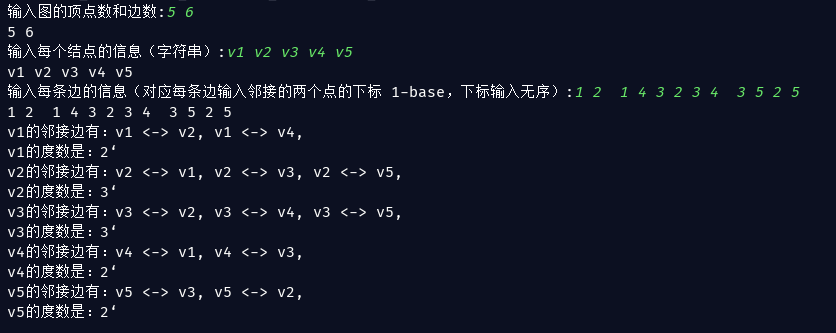
\includegraphics[width=0.8\textwidth,natwidth=400,natheight=200]{1.PNG}
        \caption{无向图的邻接边和度}
      \end{figure}

\subsection{项目2}
大致思想 :方法类似无向图。采用邻接矩阵的存储方式,Node结构体中,存放入度Indegree,出度Outdegree,结点名字data 和存放邻接点的一维数组*OutAdjList;用一个数组NodeList存储所有节点。输入每条边的信息时,将对应下标结点的信息填入。再依次打印即可
\subsubsection{实验步骤}
\begin{enumerate}
\item createAdjGraph()函数构建无向图,复杂度O(V+E),V是顶点数,E是边数。          与无向图不同的是,这里的下标输入有顺序,第一个点的信息较多,第二个点只是入度增加
\item display()打印所有顶点的所有邻接边和度数。复杂度O($V^2$),V是顶点数。       遍历每个点,对于每个点,根据度数挨个打印邻接数组中的邻接点。与无向图不同的是,当结点的出度为0时,没有邻接边。
\end{enumerate}

\subsubsection{必要代码}
\lstinputlisting[language=C++]{code/2/main.cpp }
\lstinputlisting[language=C++]{code/2/DirectedGraph.h}
\subsubsection{实验结果}如图2
	\begin{figure}[!bthp]
	\centering
        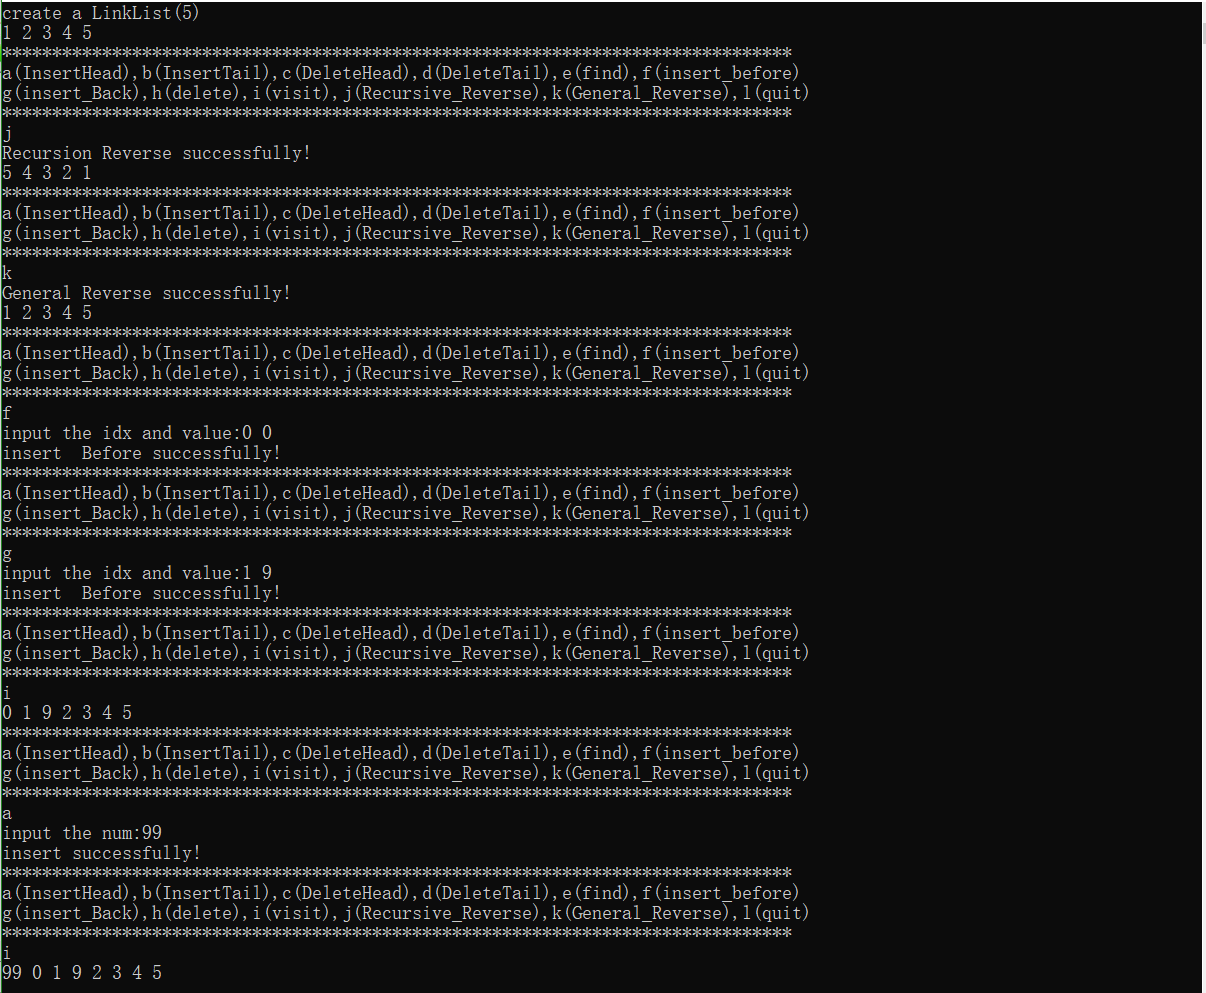
\includegraphics[width=0.8\textwidth,natwidth=400,natheight=200]{2.PNG}
        \caption{有向图的邻接边和度}
      \end{figure}

\subsection{项目3}
大致思想 :采用邻接矩阵的存储方法
\begin{enumerate}
\item BFS 是利用一个辅助队列,先访问初始结点,将初始点的 所有未访问过的邻接结点 push,再初始节点的邻居,push同理,再邻居的邻居。。。。
\item DFS就是利用一个递归,先访问出发点,再从出发点依次递归搜索出发点的每个邻接点w,若w未访问,则以 w 未新的出发点,直到最深层次的点所有邻接点都被访问了为止,再回溯到上一结点
\end{enumerate}
\subsubsection{实验步骤}
\begin{enumerate}
\item *FindAdj(int u)找邻接一维数组,复杂度O(V),V是顶点数.       先初始化Adj数组全部为0,两个点邻接时,赋邻接一维数组值为1
\item BFS(int start) 复杂度O($V^2$),V是顶点数。             每个顶点仅队列一次,出队列一次,其中对于一个顶点,遍历该顶点的每个邻接点。
\item void DFS()  复杂度O($V^2$),V是顶点数。              对图中每个顶点至多调用一次递归,一旦被标记,不再从它出发进行搜索       
\end{enumerate}
\subsubsection{必要代码}
\lstinputlisting[language=C++]{code/3/main.cpp }
\lstinputlisting[language=C++]{code/3/Graph.h}
\subsubsection{实验结果}如图3
	\begin{figure}[!bthp]
	\centering
        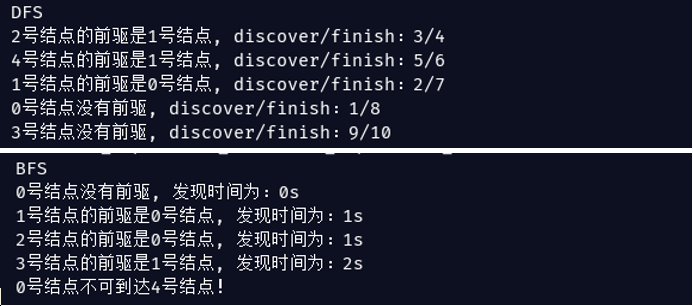
\includegraphics[width=0.8\textwidth,natwidth=400,natheight=200]{3.PNG}
        \caption{对图进行BFS 和 DFS遍历}
      \end{figure}


\subsection{项目4.1}
大致思想 :寻找关键节点:计算结点的low 值:若v存在孩子结点w,使 w.low>v.d(即w的最早访问时间在访问父亲v之后),v就是关键节点,若不是关键结点:当前结点 的相邻白色节点 与 当前结点的前驱之一 之间 有一条路径, 当前结点不是关键结点。
low值:其祖先最早能发现的时间 :即最早发现的祖先的d值。比较有三,取min:1.该结点v的访问时间d;   2.v的有回边相连的邻接灰色节点(已经访问的祖先k)的d   3.v的下一个邻接白色孩子结点的w的low值.
\subsubsection{实验步骤}
\begin{enumerate}
\item createAdjGraph(), 创建邻接矩阵,输入图的信息。复杂度O(V+E),V是顶点数,E是边数。
\item FindArticulation(), 复杂度O($V^2$),V是顶点数。             对图中每个顶点至多调用一次递归DFSArticul(Node u);
\item DFSArticul(Node u)  复杂度O($V^2$),V是顶点数。              对图中每个顶点至多调用一次递归,计算邻接孩子的low      
\end{enumerate}
\subsubsection{必要代码}
\lstinputlisting[language=C++]{code/4.1/main.cpp }
\lstinputlisting[language=C++]{code/4.1/Articulation.h }
\subsubsection{实验结果}如图4
	\begin{figure}[!bthp]
	\centering
        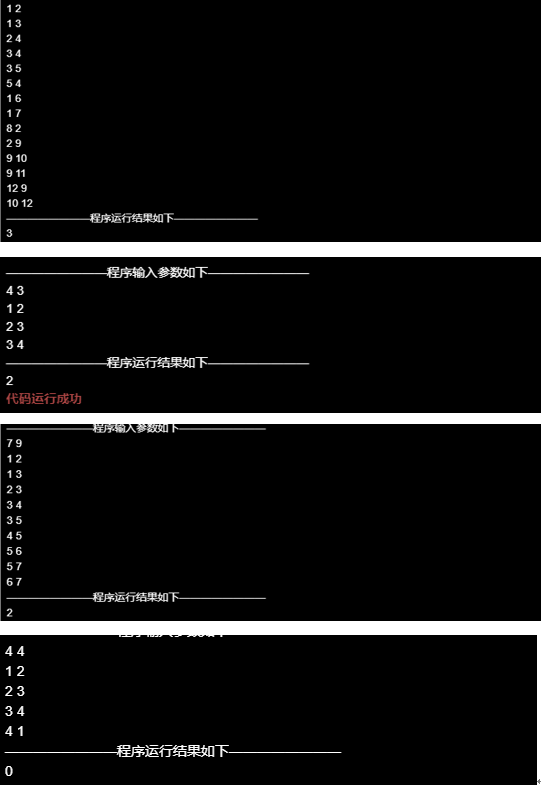
\includegraphics[width=0.8\textwidth,natwidth=400,natheight=350]{4.1.PNG}
        \caption{寻找关键结点}
      \end{figure}


\subsection{项目4.2}
大致思想 :具体的实现跟Prim类似。
  开始时将源点添加到SPT中,然后,每次增加一条边来构建SPT, 所取的边总是可以给出从源点到尚未在SPT中某个定点的最短路径。这样,顶点按照到源点的距离由小到大逐个添加到SPT中m从SPT之外的顶点中选择一个顶点v,对应边的权值最小;然后对这条边进行松弛操作。算法迭代直至图中所有顶点都在SPT中为止。
\subsubsection{实验步骤}
\begin{enumerate}
\item CreateGraph(int n, int m) 建立无负权有向图 复杂度O(V+E),V是顶点数.E是边数。      
\item Calculate\_Dijkstra(int start) 复杂度O((E+V)lgV)),V是顶点数.E是边数。           使用优先队列进行优化,一开始将所有的点除了源点之外,放到二叉堆中,然后查找节点i的时候,直接调用getTop方法,时间复杂度为O(lgn),由于对每个节点调用一次,因此总共需要V次这个操作,在获取到点i之后,通过点i进行松弛,松弛之后需要更新该节点,需要松弛的其实并非所有节点,而只是点i的临接点。因此,松弛需要调用E(图中边的数量)次,二叉堆优化后的Dijkstra算法的复杂度为O((E+V)lgV),        
\item PrintShortestPath() 复杂度O($V^2$),V是顶点数。              对每个顶点,倒序输出它的路径,直到遇到出发点为止
\end{enumerate}
\subsubsection{必要代码}
\lstinputlisting[language=C++]{code/4.2/main.cpp }
\lstinputlisting[language=C++]{code/4.2/Dijkstra.h}
\subsubsection{实验结果}如图5
	\begin{figure}[!bthp]
	\centering
        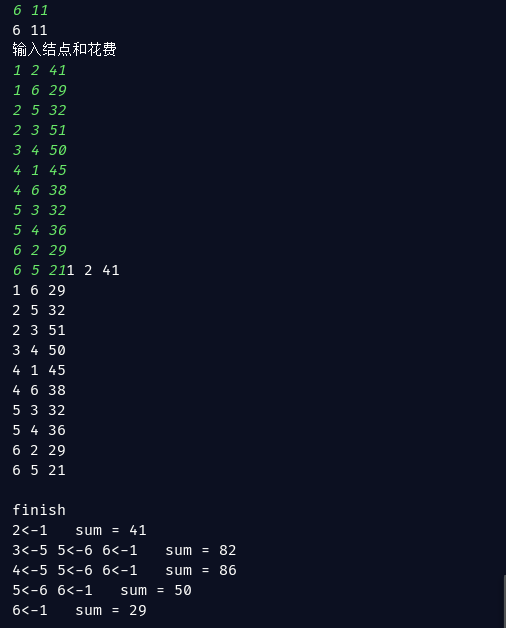
\includegraphics[width=0.8\textwidth,natwidth=400,natheight=400]{4.2.PNG}
        \caption{Dijkstra算法求单源最短路径}
      \end{figure}

\subsection{项目4.3}
大致思想 :并查集的应用。    把所有的城镇都看作一个点,每一条路都会与两个点相连接,把每个相连通的分量看成一个集合,
  然后用树来表示集合。我们只需要求出根结点的个数,就能求出有多少个集合,
  进而求出需要多少条路使它们联通,因此就可以用到并查集。
  如果是1个连通分支,说明整幅图上的点都连起来了,不用再修路了;如果是2个连通分支,
  则只要再修1条路,从两个分支中各选一个点,把它们连起来,那么所有的点都是连起来的了;
  如果是3个连通分支,则只要再修两条路……

\subsubsection{实验步骤}
\begin{enumerate}
\item normal\_find(int i),时间复杂度O(N),N是城镇个数.       根据索引,向上查找,普通单纯查找根,不压缩路径,
\item fix\_find\_recursion(int i) 最坏时间复杂度是O(m $\alpha$(N) ),N是城镇个数。其中$\alpha$是Ackerman函数的某个反函数,这个函数的值可以看成是不大于4。所以时间复杂度是线性的。           压缩路径递归查找, 往上一级找根;一直向上,直到返回值到根为止。
\item fix\_find\_non\_recursion(int x)  非递归同上
\item Merge(int p,int q) 合并操作,复杂度同上.             这里引入rank记录结点的高度,为了不增加树的高度,合并时将树的高度低的 指向 树高更 高的
\end{enumerate}
\subsubsection{必要代码}
\lstinputlisting[language=C++]{code/4.3/main.cpp }
\lstinputlisting[language=C++]{code/4.3/BuildPathToMerge.h}
\subsubsection{实验结果}如图6
	\begin{figure}[!bthp]
	\centering
        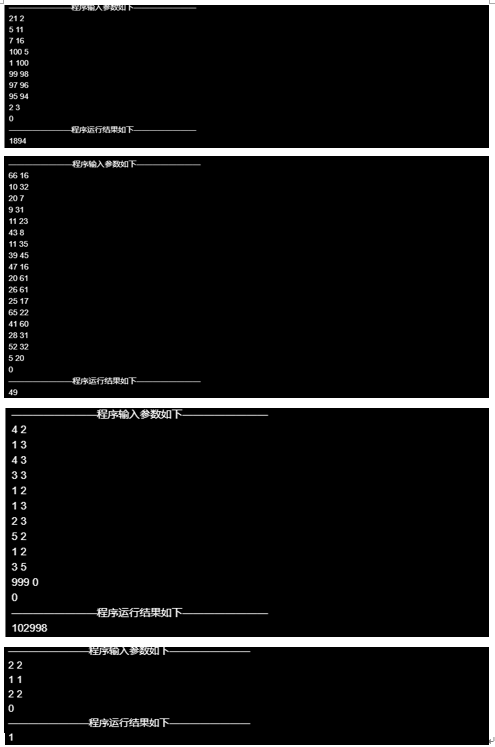
\includegraphics[width=0.8\textwidth,natwidth=400,natheight=450]{4.3.PNG}
        \caption{并查集的应用:需要再修几条公路}
      \end{figure}

\subsection{项目4.4}
大致思想 :求最小生成树:kruskal算法. 求可以使任意两个村庄连通的最小公路总长度,即求最小生成树。
 Kruskal算法是基于贪心的思想得到的。首先我们把所有的边按照权值先从小到大排列,
 接着按照顺序选取每条边,如果这条边的两个端点不属于同一集合,那么就将它们合并,
 直到所有的点都属于同一个集合为止。至于怎么合并到一个集合,
 可以用到一个工具:并查集。
 换而言之,Kruskal算法就是基于并查集的贪心算法。

\subsubsection{实验步骤}
\begin{enumerate}
\item 算法描述:1.1将图G看做一个森林,每个顶点为一棵独立的树。1.2将所有的边加入集合S,即一开始S = E。1.3从S中拿出一条最短的边(u,v)此处使用优先队列,如果(u,v)不在同一棵树内,则连接u,v合并这两棵树,同时将(u,v)加入生成树的边集E'。1.4重复1.3直到所有点属于同一棵树,边集E'就是一棵最小生成树。
\item 并查集的时间复杂度项目 4.3 已经分析,这里不再赘述
\item  kruskal()计算最小公路长度  。时间复杂度O(V*((m $\alpha$(V))+lgE )),V是顶点数,E是图中边的条数。              因为采用优先队列,每次取最短的边,复杂度lgE。加上Merge 的复杂度,对于这两个操作,需要进行到所有顶点都连通且不成环,即V-1次。所以得到复杂度。
\end{enumerate}
\subsubsection{必要代码}
\lstinputlisting[language=C++]{code/4.4/main.cpp }
\lstinputlisting[language=C++]{code/4.4/Kruskal.h}
\subsubsection{实验结果}如图7
	\begin{figure}[!bthp]
	\centering
        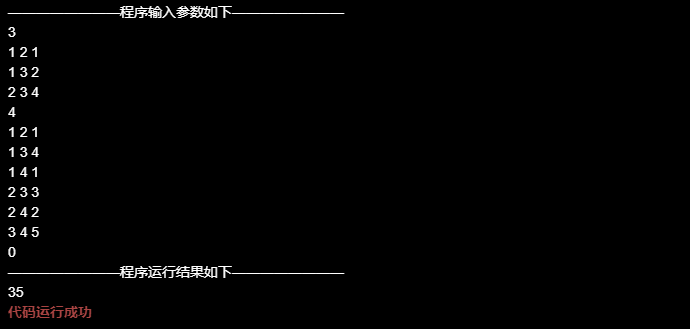
\includegraphics[width=0.8\textwidth,natwidth=400,natheight=90]{4.4.PNG}
        \caption{求最小生成树的kruskal算法求连通所修最短公路长度}
      \end{figure}

\section{实验总结}详情请关注我的GitHub:DarringZhang

\end{document}
